\section{Machine Learning}

\begin{itemize}
\item What is machine learning?
\item Supervised learning, i.e.\ have labelled data.
\item Binary classification tasks: Every training example has a label indicating
  the class membership.
\item In HEP, the positive class is typically referred to as \emph{signal} while
  the negative class is referred to as \emph{background}.
\item What is training data, etc.
\item What is training.
\end{itemize}


\subsection{Boosted Decision Trees}

Boosted decision trees (BDT) are a classification algorithm consisting on an
ensemble of \emph{decision trees} that are combined to yield a powerful
classifier. The ensemble of decision trees is created using a algorithm referred
to as \emph{boosting}, which iteratively constructs decision tree classifiers or
regressors while emphasising training examples that were incorrectly classified
in prior iterations. The following description of BDT focuses on the algorithm
implemented in \textsc{TMVA}~\cite{TMVA}, which is used in this thesis for the
training of BDTs.


Classification and regression trees~\cite{Breiman:1984jka,hastie09}, hereafter
collectively referred to as \emph{decision trees}, are used as base functions in
BDTs. A decision tree partitions a multivariate space with coordinates
$\myvec{x} = (x_1, \dots, x_n)$ by recursively performing binary splits along
the coordinate axes until a stopping criterion is met. The resulting binary tree
structure and partitioning is illustrated in \Cref{fig:decision_tree} for a
two-dimensional example. A decision tree with $J$~leaf nodes partitions the
input space into $J$~disjoint subregions denoted by $R_j$ for $j = 1, \dots,
J$. A constant value $c_j$ is assigned to every region $R_j$ such that the
prediction of a decision tree can be written as~\cite{hastie09}
\begin{align*}
  f(\myvec{x}) = \sum_{j = 1}^{J} c_j \, \mathbf{1}(\myvec{x} \in R_j) \qquad \text{with} \qquad \mathbf{1}(\myvec{x} \in R_j) =
  \begin{cases}
    1, & \myvec{x} \in R_j \\
    0, & \text{else}
  \end{cases} \,\text{.}
\end{align*}

\begin{figure}[htbp]
  \centering

  \begin{subfigure}[b]{0.46\textwidth}
    \centering
    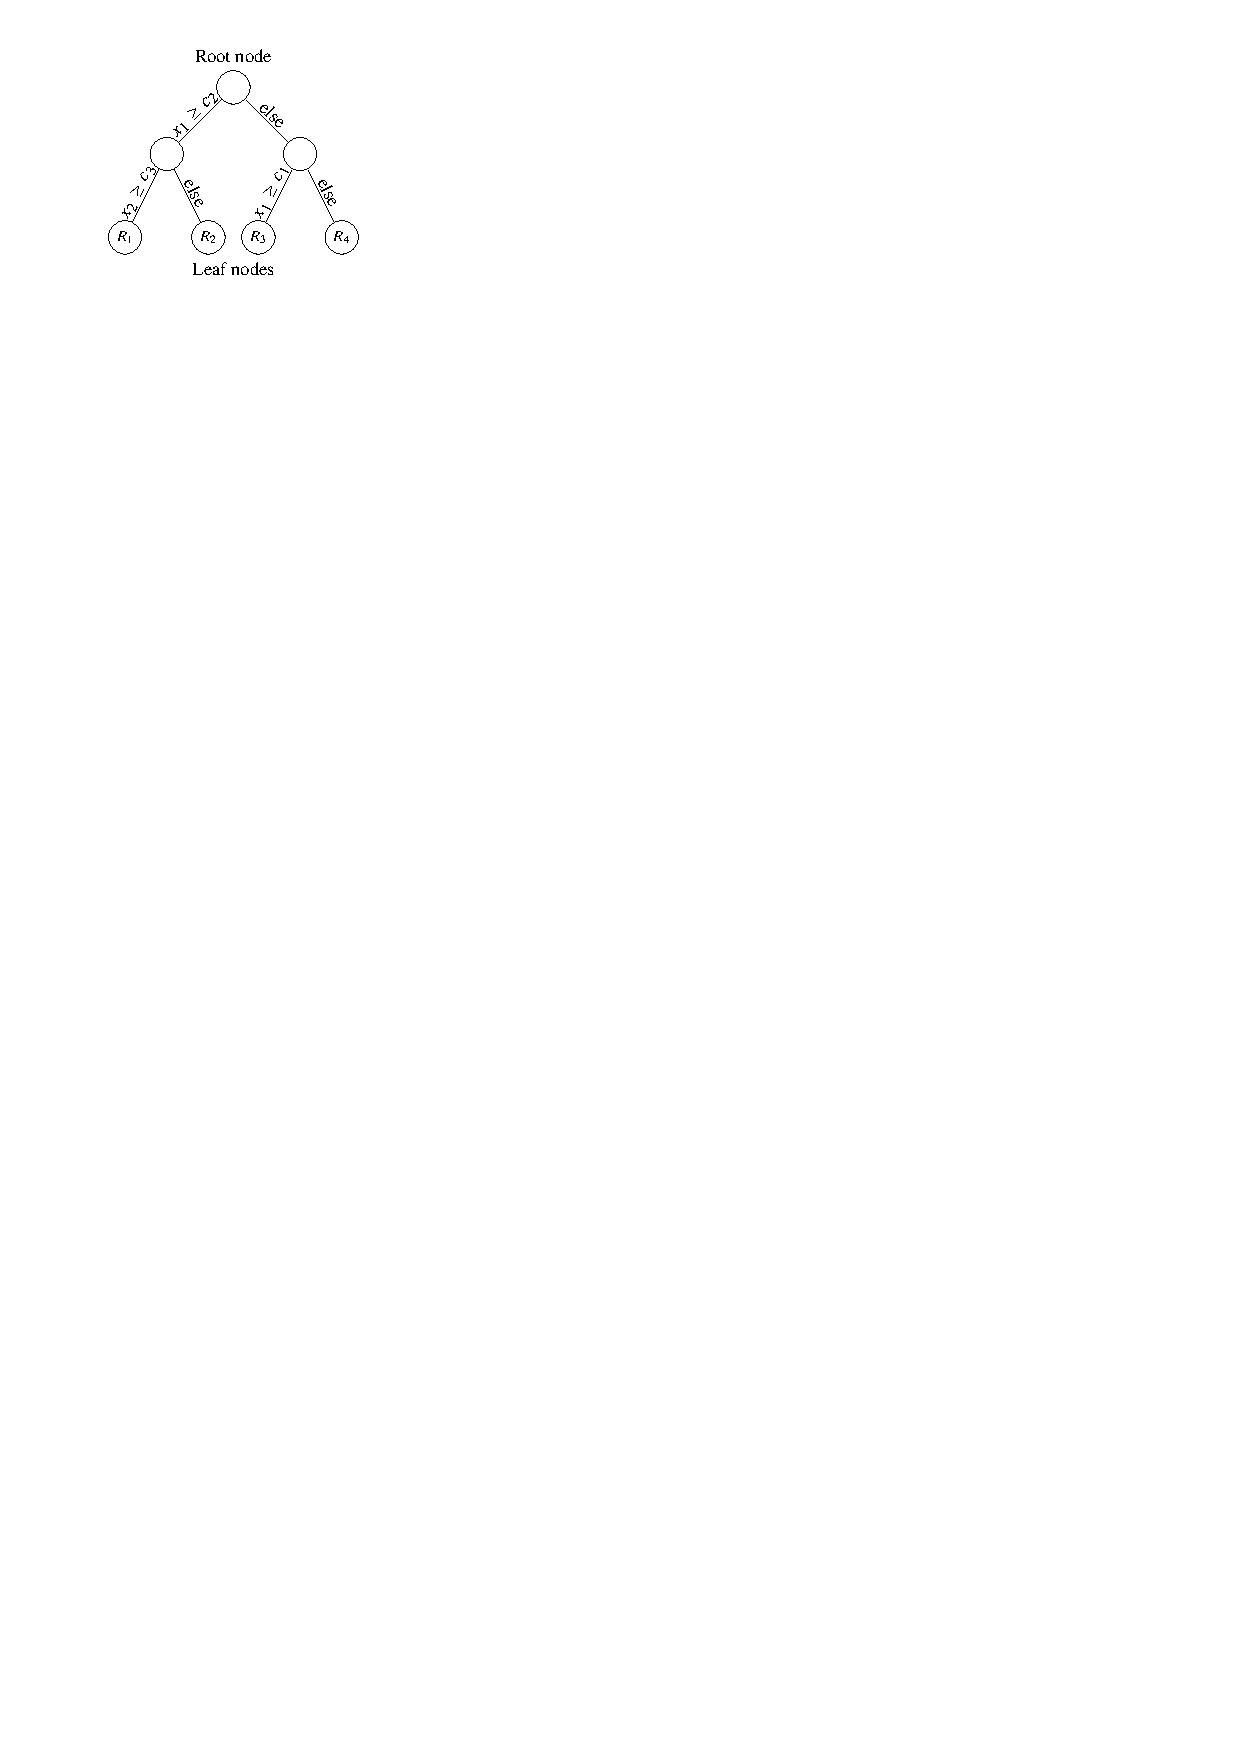
\includegraphics[scale=1.05]{ml/decision_tree}
    \caption{Binary tree structure of a decision tree.}
  \end{subfigure}\hfill%
  \begin{subfigure}[b]{0.46\textwidth}
    \centering
    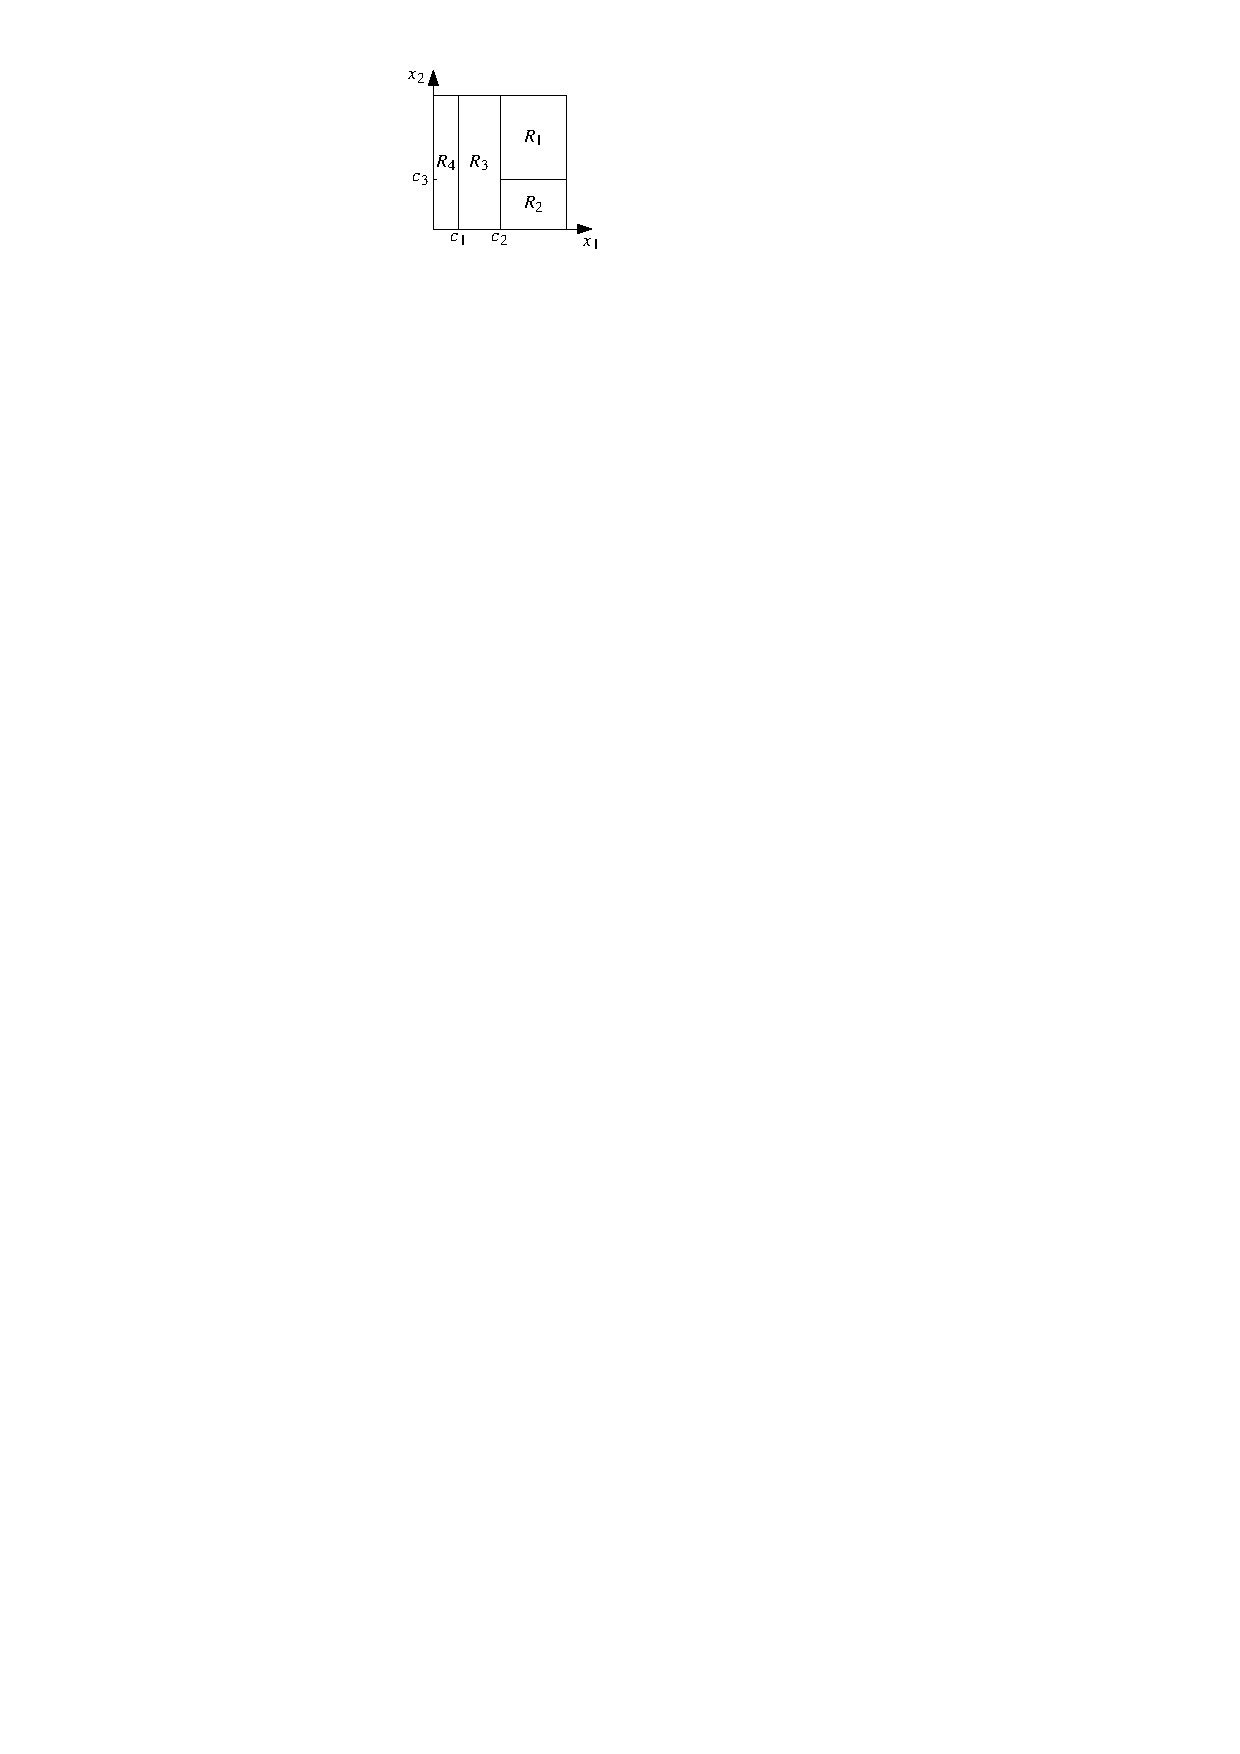
\includegraphics[scale=1.05]{ml/decision_tree_partitioning}
    \vspace*{0.7em}
    \caption{Partitioning resulting from the binary tree in (a).}
  \end{subfigure}\hfill%

  \caption{Example of a decision tree in a two-dimensional space with
    coordinates $\myvec{x} = (x_1, x_2)$. The tree has a depth of two resulting
    in four leaf nodes that define the regions $R_1, \dots, R_4$. The figure is
    adapted from Ref.~\cite{hastie09}.}%
  \label{fig:decision_tree}
\end{figure}

Classification trees are constructed such that the partitioning of the input
space yields subregions with low impurity, that is, the regions are mostly
populated by training examples of a single class. In this case, the impurity of
a tree node is quantified by the Gini index
\begin{align*}
  I_{\text{G}}(p) = 2 p (1 - p) \,\text{,}
\end{align*}
where $p$ is the proportion of examples from the positive class in a given
node~\cite{hastie09}. A \emph{greedy} strategy is adopted to grow decision trees
by performing the best possible split at every node. This split is determined by
minimising the weighted sum of Gini impurities of the resulting daughter nodes,
where impurities are weighted according to the total weight of training examples
populating a given node. In the classification case, the constants $c_j$
assigned to leaf nodes of the tree are either--depending on the algorithm
configuration--the proportion of examples from the positive class or the class
label of the majority class.

Regression trees are constructed using a similar approach, however, with an
altered splitting criterion and different assigment of constants to leaf
nodes. Consider the split of a parent node into a left (L) and right (R)
daughter node. Let $(y, w)$ denote the tuple of regression target and weight for
a given training example. Moreover, let $T_{\text{L}}$ and $T_{\text{R}}$ denote
the set of $(y, w)$ for training examples populating the left and right daughter
node, respectively. The constants $c_{\text{L}}$ and $c_{\text{R}}$ assigned to
the daughter nodes are given by
\begin{align*}
  c_{\text{L}} = \frac{\sum_{(y, w) \in T_{\text{L}}} w y}{\sum_{(y, w) \in T_{\text{L}}} w} \qquad \text{and} \qquad c_{\text{R}} = \frac{\sum_{(y, w) \in T_{\text{R}}} w y}{\sum_{(y, w) \in T_{\text{R}}} w} \,\text{,}
\end{align*}
which is the weighted mean of the regression target for the training examples
populating the left and right node, respectively. The best possible split in a
regression tree is chosen such that the squared error defined as
\begin{align*}
  \sum_{(y, w) \in T_{\text{L}}} w (y - c_{\text{L}})^2 + \sum_{(y, w) \in T_{\text{R}} } w (y - c_{\text{R}})^2
\end{align*}
is minimised.






Booooooooostiiing... yeah!



\textsc{TreeBoost} by Friedman~\cite{Friedman:2001wbq}


\subsection{Neural Networks}

\subsubsection{Recurrent Neural Networks}%
\label{sec:rnn}


%%% Local Variables:
%%% mode: latex
%%% TeX-master: "../../phd_thesis"
%%% End:
